\section{Úvod}
Následující dokument popisuje způsob implementace kompilátoru z~jazyka IFJ17 do mezikódu
IFJcode17 ve variantě 2. Jedná se o~projekt,
který byl vyprácován podle zadání do předmětů IFJ a IAL na Fakultě
informačních technologí Vysokého učení technického v~Brně.

Dokumentace popisuje způsob řešení, dekompozici překladače na jednotlivé moduly,
popis použitých algoritmů a datových struktur a způsob práce v~týmu.

\section{Teoretický rozbor}
Naším úkolem bylo implementovat překladač jazyka IFJ17 (který je podmnožinou jazyka známého jako \mbox{FREEBASIC})
do mezikódu IFJcode17. Program čte zdrojový kód ze standardního vstupu a v~případě překladu bez chyby generuje cílový
kód. V~případě chyby je navrácen odpovídající chybový kód a vytisknuta informace o~typu chyby. Varianta 2 specifikuje
zadání na užití tabulky s~rozptýlenými položkami při implementaci tabulky symbolů.

Pro běh překladače byl použit tzv. \textbf{Syntaxí řízený překlad}, což předurčuje syntaktický analyzátor k~řízení činnosti
celého překladače. SA tedy získává vstupní tokeny a kontroluje, zda tvoří řetězec generovaný
LL gramatikou, spouští sémantické kontroly a řídí konstrukci kódu.
Optimalizátor poté pracuje mimo hlavní zpracování, je spuštěn po syntaktické analýze nad vygenerovaným kódem.

Implementace překladače se nám tedy rozpadla na následující moduly:
\begin{itemize}
    \item Lexikální analyzátor
    \item Syntaktický analyzátor
    \item Sémantický analyzátor,
    \item Generátor cílového kódu
    \item Optimalizátor kódu
\end{itemize}

Jelikož výstupem překladu je jistá forma mezikódu, používáme metodu generování tohoto kódu přímo ze syntaktické analýzy \textbf{bez generování abstraktního syntaktického stromu} nebo zásobníkového kódu.

Propojení jednotlivých komponent naznačuje následující schéma:
\vspace*{4px}
\begin{figure}[htbp]
	\centering
	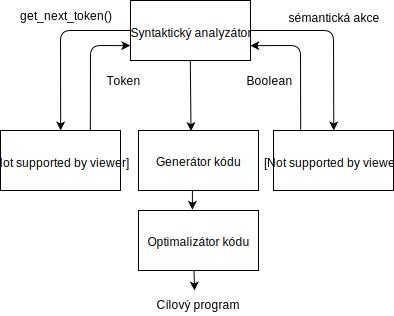
\includegraphics[width=0.65\textwidth, angle=0]{src/assets/structure.pdf}
\end{figure}